\documentclass[tikz, border=10pt]{standalone}
\usepackage{tikz}
\usetikzlibrary{positioning, arrows.meta, calc, backgrounds, fit, shapes.geometric}

\begin{document}
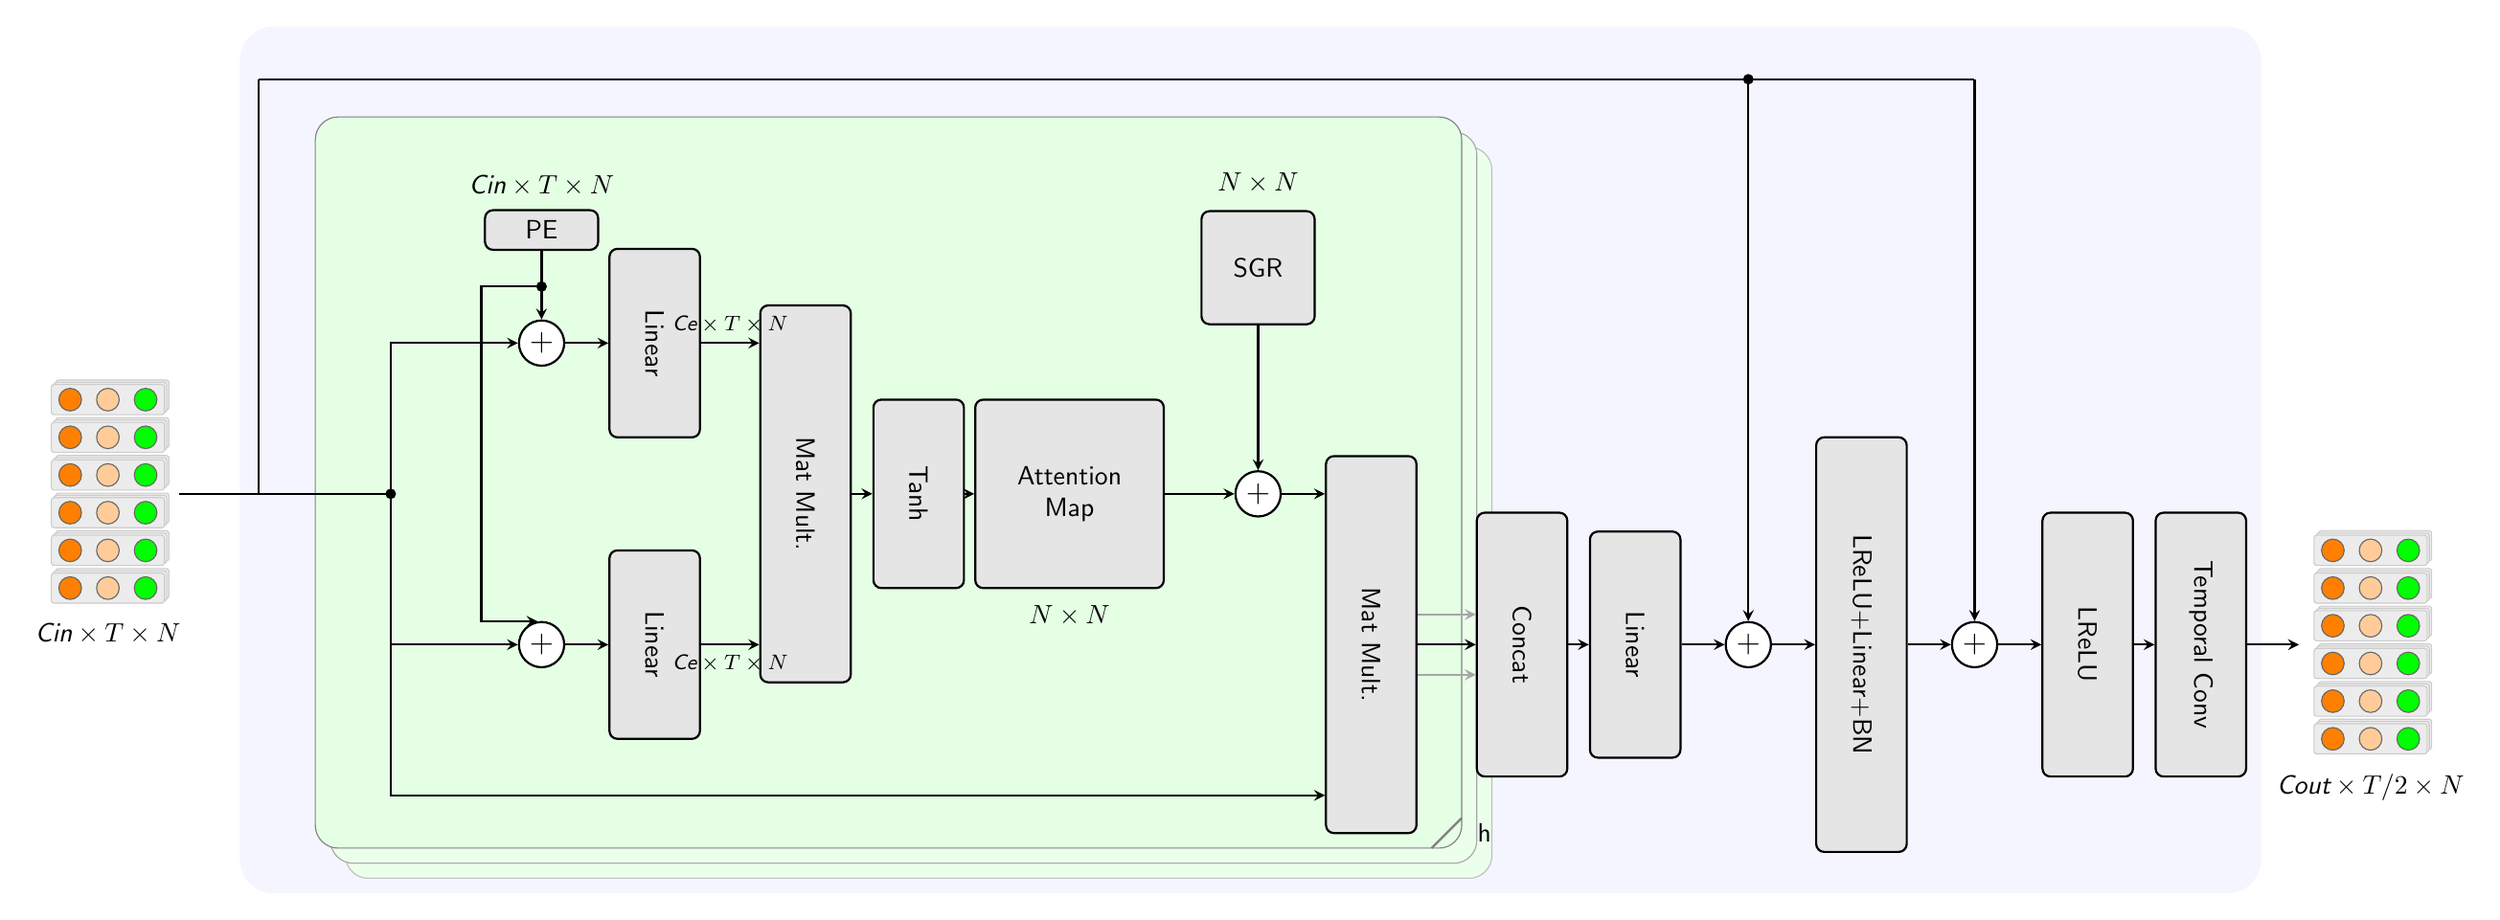
\begin{tikzpicture}[
    font=\sffamily,
    box/.style = {draw=black, rounded corners=3pt, fill=gray!20, thick, align=center, inner sep=4pt},
    sum/.style = {draw=black, circle, thick, fill=white, inner sep=1pt, minimum size=0.6cm, font=\large},
    arr/.style = {->, >=stealth, thick},
    line/.style = {-, thick}
]

    % ==========================================
    % Custom Macro for Input/Output Tensors
    % ==========================================
    \newcommand{\drawtensor}[3]{
        % #1 = x, #2 = y, #3 = label
        \begin{scope}[shift={(#1,#2)}]
            % Back plates for depth
%             \filldraw[fill=gray!15, draw=gray!40, rounded corners=1pt] (0.2, 0.2) rectangle (1.7, 3.2);
%             \filldraw[fill=gray!15, draw=gray!40, rounded corners=1pt] (0.1, 0.1) rectangle (1.6, 3.1);
%             \filldraw[fill=gray!15, draw=gray!40, rounded corners=1pt] (0, 0) rectangle (1.5, 3);
            % Circles
            \foreach \y in {0.25, 0.75, 1.25, 1.75, 2.25, 2.75} {
	            \foreach \yy in {0.06, 0.03, 0} {
		\filldraw[fill=gray!15, draw=gray!40, rounded corners=1pt] (\yy,\y - 0.2 + \yy) rectangle (1.5 + \yy, \y + 0.2 + \yy);
		%\filldraw[fill=gray!15, draw=gray!40, rounded corners=1pt] (0, \y - 0.2) rectangle (1.5, \y + 0.2);
		}
                \filldraw[fill=orange, draw=black!60] (0.25, \y) circle (0.15);
                \filldraw[fill=orange!40, draw=black!60] (0.75, \y) circle (0.15);
                \filldraw[fill=green, draw=black!60] (1.25, \y) circle (0.15);
            }
            % Label
            \node[below] at (0.75, -0.1) {#3};
        \end{scope}
    }

    % ==========================================
    % Main Layout Coordinates & Nodes
    % ==========================================

    % Input Tensors
    \drawtensor{-5.5}{-3.0}{$\textit{Cin} \times T \times N$}

    % Input Splits
    \coordinate (in_start) at (-3.8, -1.5);
    \coordinate (p1) at (-2.75, -1.5); % Main bypass split point
    \coordinate (in_split) at (-1, -1.5); % Inner green block split point

    % Top Bypass Line
    \draw[line] (in_start) -- (p1);
    %\fill (p1) circle (2pt);
    \draw[line] (p1) -- (-1, -1.5);
    \draw[line] (p1) -- (-2.75, 4.0);
    \draw[line] (-2.75, 4.0) -- (17, 4.0);

    % Inner Block Nodes (Green region)
    \fill (in_split) circle (2pt);

    \node[sum] (sum1) at (1, 0.5) {$+$};
    \node[sum] (sum2) at (1, -3.5) {$+$};

    \node[box, minimum height=0.5cm, minimum width=1.5cm] (pe) at (1, 2) {PE};
    \node[above=0.05cm of pe] {$\textit{Cin} \times T \times N$};

    % Linear Layers (rotated text)
    \node[box, minimum height=2.5cm, minimum width=1.2cm] (lin1) at (2.5, 0.5) {\rotatebox{-90}{Linear}};
    \node[box, minimum height=2.5cm, minimum width=1.2cm] (lin2) at (2.5, -3.5) {\rotatebox{-90}{Linear}};

    % Mat Mult 1
    \node[box, minimum height=5cm, minimum width=1.2cm] (mat1) at (4.5, -1.5) {\rotatebox{-90}{Mat Mult.}};

    % Tanh & Attention Map
    \node[box, minimum height=2.5cm, minimum width=1.2cm] (tanh) at (6, -1.5) {\rotatebox{-90}{Tanh}};
    \node[box, minimum height=2.5cm, minimum width=2.5cm] (attn) at (8, -1.5) {Attention\\Map};
    \node[below=0.1cm of attn] {$N \times N$};

    % SGR & Sum 3
    \node[sum] (sum3) at (10.5, -1.5) {$+$};
    \node[box, minimum height=1.5cm, minimum width=1.5cm] (sgr) at (10.5, 1.5) {SGR};
    \node[above=0.1cm of sgr] {$N \times N$};

    % Mat Mult 2
    \node[box, minimum height=5cm, minimum width=1.2cm] (mat2) at (12, -3.5) {\rotatebox{-90}{Mat Mult.}};

    % Right Side Sequence Nodes
    \node[box, minimum height=3.5cm, minimum width=1.2cm] (concat) at (14, -3.5) {\rotatebox{-90}{Concat}};
    \node[box, minimum height=3cm, minimum width=1.2cm] (lin3) at (15.5, -3.5) {\rotatebox{-90}{Linear}};
    \node[sum] (sum4) at (17, -3.5) {$+$};
    \node[box, minimum height=5.5cm, minimum width=1.2cm] (lrelu_bn) at (18.5, -3.5) {\rotatebox{-90}{LReLU+Linear+BN}};
    \node[sum] (sum5) at (20, -3.5) {$+$};
    \node[box, minimum height=3.5cm, minimum width=1.2cm] (lrelu) at (21.5, -3.5) {\rotatebox{-90}{LReLU}};
    \node[box, minimum height=3.5cm, minimum width=1.2cm] (temp_conv) at (23, -3.5) {\rotatebox{-90}{Temporal Conv}};

    % Output Tensor
    \drawtensor{24.5}{-5.0}{$\textit{Cout} \times T/2 \times N$}

    % ==========================================
    % Routing Paths
    % ==========================================

    % Inner Splits
    \draw[arr] (in_split) |- (sum1.west);
    \draw[arr] (in_split) |- (sum2.west);

    % Bottom Bypass to Mat2
    \draw[line] (in_split) |- (-0.5, -5.5);
    \draw[arr] (-0.5, -5.5) -- (mat2.west |- 0,-5.5);

    % PE splits
    \draw[arr] (pe.south) -- (sum1.north);
    \fill (1, 1.25) circle (2pt);
    \draw[arr] (1, 1.25) -- (0.2, 1.25) |- (sum2.100);

    % Forward passes through green block
    \draw[arr] (sum1.east) -- (lin1.west);
    \draw[arr] (sum2.east) -- (lin2.west);

    \draw[arr] (lin1.east) -- (mat1.west |- lin1.east) node[midway, above] {\footnotesize $\textit{Ce} \times T \times N$};
    \draw[arr] (lin2.east) -- (mat1.west |- lin2.east) node[midway, below] {\footnotesize $\textit{Ce} \times T \times N$};

    \draw[arr] (mat1.east) -- (tanh.west);
    \draw[arr] (tanh.east) -- (attn.west);
    \draw[arr] (attn.east) -- (sum3.west);
    \draw[arr] (sgr.south) -- (sum3.north);
    \draw[arr] (sum3.east) -- (mat2.west |- sum3.east);

    % Multi-head out to Concat
    \draw[arr, draw=gray!70] ($(mat2.east)+(0, 0.4)$) -- ($(concat.west)+(0, 0.4)$);
    \draw[arr] (mat2.east) -- (concat.west);
    \draw[arr, draw=gray!70] ($(mat2.east)+(0, -0.4)$) -- ($(concat.west)+(0, -0.4)$);

    % Right Side Sequence Routing
    \draw[arr] (concat.east) -- (lin3.west);
    \draw[arr] (lin3.east) -- (sum4.west);
    \draw[arr] (sum4.east) -- (lrelu_bn.west);
    \draw[arr] (lrelu_bn.east) -- (sum5.west);
    \draw[arr] (sum5.east) -- (lrelu.west);
    \draw[arr] (lrelu.east) -- (temp_conv.west);
    \draw[arr] (temp_conv.east) -- (24.3, -3.5);

    % Top Bypass Drop-downs
    \fill (17, 4.0) circle (2pt);
    \draw[arr] (17, 4.0) -- (sum4.north);
    \draw[line] (17, 4.0) -- (20, 4.0);
    \draw[arr] (20, 4.0) -- (sum5.north);

    % ==========================================
    % Background Enclosures
    % ==========================================
    \pgfdeclarelayer{bg}
    \pgfsetlayers{bg,main}

    \begin{pgfonlayer}{bg}
        % 1. Light Blue Enclosure (Outer)
        \fill[blue!4!white, rounded corners=3ex] (-3.0, 4.7) rectangle (23.8, -6.8);

        % 2. Green Enclosures (Heads / Inner) - rendered back to front
        \def\gtl{-2.0} \def\gtop{3.5} \def\gbr{13.2} \def\gbot{-6.2}

        % Back Head
        \filldraw[fill=green!8, draw=black!25, rounded corners=2ex]
            (\gtl+0.4, \gtop-0.4) rectangle (\gbr+0.4, \gbot-0.4);
        % Mid Head
        \filldraw[fill=green!8, draw=black!35, rounded corners=2ex]
            (\gtl+0.2, \gtop-0.2) rectangle (\gbr+0.2, \gbot-0.2);
        % Front Head
        \filldraw[fill=green!10, draw=black!50, rounded corners=2ex]
            (\gtl, \gtop) rectangle (\gbr, \gbot);

        % Small "h" marker cut
        \draw[black!50, thick] (\gbr-0.4, \gbot) -- (\gbr, \gbot+0.4);
        \node at (\gbr+0.3, \gbot+0.2) {h};

    \end{pgfonlayer}

\end{tikzpicture}
\end{document}
